\section{I/O Burst Buffer Model}

%\begin{figure}[tb]
%	\centering
%	\includegraphics
%	\caption{definition}
%	\label{definition}
%\end{figure}

Throughput-based Model, Cost-based Model and buffer queue write back model will be described in this section.
Throughput-based Model compare one-side buffer throughput with two-side buffer, cost-based model compare one-side buffer cost with two-side buffer, and buffer queue write back model. 
We make definitions shows in Table.~\ref{definition} in order to describe our model:
\begin{table}[tb]
	\caption{Definition of parameters}
	\label{definition}
\begin{tabular}{|p{3cm}|p{5cm}|}
	\hline
	$c_1,c_2$&Numbers of computing nodes in system 1 and system 2\\\hline
	$n_1, n_2$&Numbers of I/O buffer nodes in system 1 and system 2.\\\hline
	$m_1,m_2$&Available memory size for each I/O node in system 1 and 2, also the maximum buffer size will be $n_1\times m_1$ and $n_2\times m_2$\\\hline
	$D_1(n_2),D_2(n_2)$&Throughput when $n_2$($n_1$) I/O nodes in system 1 (system 2) connect to storage in the other system directly, here we assume only I/O nodes in each system have Internet connection.\\\hline
	$I(n_1,n_2)$& 	Internet throughput using $n_1,n_2$ I/O buffer nodes respectively, Since overall Internet throughput is affected by number of nodes involved in connection.\\\hline
	$E_1(n_1), E_2(n_2)$&Interconnection network throughput in system 1 and 2, although interconnection throughput is also affected by numbers of I/O nodes and computing nodes, numbers of users will running application on different number of computing nodes.\\\hline
	%, it is difficult to compute each throughput, so here we use $E_1(n_1)$ to refer to limitation of maximum throughput of interconnection network in system 1 with $n_1$ I/O nodes, likely ,$E_2(n_2)$ is limitation of maximum throughput of interconnection network in system 2 with $n_2$ I/O nodes.
	$M_1(n_1),M_2(n_2)$& Throughput of connection between storage and $n_1$ I/O nodes in system 1 and storage and $n_2$ I/O nodes in system 2.\\\hline
	$C_1\_Money(T)$,$C_2\_Money(T)$& Cost for standard node in system 1 and 2 for $T$ time usage\\\hline
	%and cost for node in system 1 is $C_2\_Money(T)$ for $T$ time usage, and since I/O nodes may use a better network, 
	$C_1\_High\_Money(T)$,$C_2\_High\_Money(T)$& cost I/O nodes in system 1 and 2 for $T$ time usage, since I/O nodes may use a better network condition, we assume it will cost more than normal nodes.\\\hline
\end{tabular}
\end{table}

\subsection{Throughput-based Model}
%There are many facts will affect throughput of Internet, so here a moniter is used to evaluate throughput between 
In the case of one-side buffer, there are two data transfers: computation nodes to I/O buffer nodes in system 2, I/O buffer nodes in system 2 to storage in system 1, so throughput will be:
\begin{equation}
	\text{throughput}_{\text{one-side}}=\min\{D_1(n_2),E_2(n_2)\} \label{throughput1}
\end{equation}

In the case of two-side buffer, there are three data transfers: computation nodes to I/O buffer nodes in system 2, I/O buffer nodes in system 2 to I/O buffer nodes in system 1, I/O buffer nodes in system 1 to storage in system 1, throughput will be:

\begin{equation}
	\text{throughput}_{\text{two-side}}=\min\{M_1(n_1),I(n_1,n_2),E_2(n_2)\} \label{throughput2}
\end{equation}

In this throughput-based model, these two throughputs are evaluated, and a switch is based on these two values:

\begin{equation}
	\begin{cases}
		\text{throughput}_{\text{one-side}} \geq \text{throughput}_{\text{two-side}} & \text{use one-side}\\
		\text{throughput}_{\text{one-side}} < \text{throughput}_{\text{two-side}} & \text{use two-side}
	\end{cases}
\end{equation}

\subsection{Cost-based Model}
In the case of cost-based model, we consider
using \ref{throughput1},and \ref{throughput2} total time for transferring unit size of data can be compute as:

\begin{equation}
	\begin{cases}
		T_1=\frac{1}{\min\{D_1(n_2),E_2(n_2)\}} & \text{one-side}\\
		T_2=\frac{1}{\min\{M_1(n_1),I(n_1,n_2),E_2(n_2)\}} &\text{two-side}
	\end{cases}
\end{equation}

here we compute cost by using $T_1,T_2$:
\begin{equation}
	\text{cost}_\text{one-side}=c_2\times C_2\_Money(T_1)+n_2\times C_2\_High\_Money(T_1)
\end{equation}
\begin{align}
	\text{cost}_\text{two-side}&=c_2\times C_2\_Money(T_2)\\\nonumber 
				     &+n_1\times C_1\_High\_Money(T_2)\\ \nonumber
				     &+n_2\times C_2\_High\_Money(T_2)
\end{align}

In this throughput-based model, these two throughput are evaluated, and a switch is based on these two values:

\begin{equation}
	\begin{cases}
		\text{cost}_{\text{one-side}} \geq \text{cost}_{\text{two-side}} & \text{use one-side}\\
		\text{cost}_{\text{one-side}} < \text{cost}_{\text{two-side}} & \text{use two-side}
	\end{cases}
\end{equation}

%\subsection{}
%\subsection{Migration Model}
%Since there are some condition that some supercomputer nodes must be shut down, and jobs running on these nodes have to be migrate to another cloud. There are 
%\begin{equation}
%	Data	
%\end{equation}
\subsection{Buffer Queue Write Back Model}

\begin{figure}[tb]
	\centering
	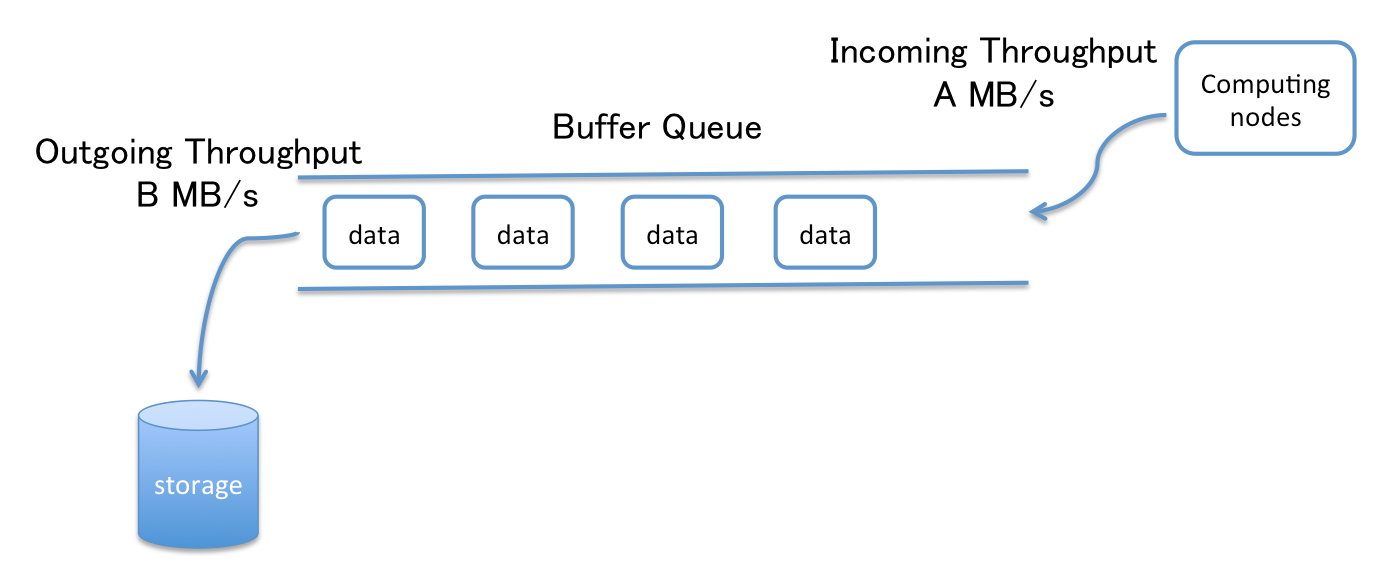
\includegraphics[width=6cm]{buffer_queue}
	\caption{buffer queue}
	\label{buffer queue}
\end{figure}

If the buffer size is unlimited. then we can buffer all data in the I/O buffer nodes, and achieve a high throughput in cloud burst.
However buffer size can not be unlimited, we can not buffer all data in the I/O buffer nodes, data in buffer nodes have to be write back to storage in another system.
The problem is which data should be written back to storage, like cache in cpu, if we can reduce cache miss in this situation, we can increase throughput. 
According to data locality, we use a priority queue to determine which data should be write back.

Consider Fig.~\ref{buffer queue}, assume average incoming throughput is A MB/s and average outgoing throughput is B MB/s, if A always larger than B, after $T$ time buffer queue will full.
\[T=\frac{m_2\times n_2}{A-B}\]

After that, since buffer queue is full, I/O server can not send more data to I/O buffer nodes, have to block any read and write request since that.
In this case, jobs running on public cloud have to be moved back to original system until buffer queue is empty.
